%!TEX root = ../../thesis.tex


\section{Synthetic Stellar models of cool stars}
The understanding of stellar physics is strongly built upon modelling, incorporating stellar structure, atmospheres and evolution, pieced together with several physical, chemical and hydrodynamical models.
One particular model output of importance for this work are the synthetic stellar spectra.
These spectra can be compared to observed spectra to attempt to classify and understand the stellar populations, as well as test the models fit to reality.
There is an ever evolving effort to improve these stellar models and synthetic spectra to better match the observations; incorporating more physics, chemical reactions, line lists, and using the latest element abundances.
This work extensively uses the {PHOENIX-ACES} synthetic spectra, with a little experimentation with the {BT-Settl} models.
A collection of several theoretical stellar spectral libraries can be found at the Spanish Virtual Observatory \href{http://svo2.cab.inta-csic.es/theory/newov/index.php}{Theoretical Spectra Web Server}.

The~\citet{kurucz_model_1979} models are popular synthetic models for stars ranging between G-O type with effective temperatures between 5500--50\,000\K{}.
For cooler stars, M-dwarfs and even Brown Dwarfs the stellar models are based on the {PHOENIX} code~\citep[e.g.][]{hauschildt_parallel_1997}.
Initially created for studying the ejecta of Novae it was \emph{Extended} to low mass stars and Brown Dwarfs~\citep{allard_model_1995}.
The {PHOENIX} modelling code has evolved over time incorporating new physical models to better explain the atmospheres.
The \emph{NextGen} models~\citep{hauschildt_nextgen_1999} treated the stellar atmosphere as a gas in chemical equilibrium, but the resulting spectra for very low mass stars was poor due to no treatment of dust in the stellar atmospheres.

The~\citet{allard_limiting_2001} \emph{COND} and \emph{DUSTY} models both investigate the extreme limits of clouds in the atmospheres of cool stars.
They include condensation physics (Gibbs free energy, gas partial pressures etc.) into the chemical equilibrium model, as well as the optical interaction of light with the dust/condensates (dust opacities and scattering).
The \emph{DUSTY} models simulate `inefficient/no settling' where condensation/dust forms and stays in the atmosphere and it affects the spectrum through the dust opacities.
At the other extreme the \emph{COND} models ignore the dust opacities and simulate `efficient settling', in which all the condensates and dust clouds fall below the spectrum forming region.

The treatment of clouds and dust is important for the modelling of low mass stars and Brown Dwarfs.
The \emph{DUSTY}/\emph{COND} models are similar above 2600\K{} but below this temperature they diverge due to the crystallization of silicates in the atmosphere~\citep{allard_limiting_2001}.
These are only a few of the physical considerations implemented in the synthetic models.
The other notable changes are due to use of specific line lists used.
The models beginning with {AMES} use the {NASA-AMES} \ce{H2O} and \ce{TiO} line lists, while the {BT} models use the~\citet{barber_highaccuracy_2006} \ce{H2O} line list.
Between models the use of improved solar abundance measurements is also included~\citep[][]{asplund_chemical_2009}.

In this work synthetic spectral from the {PHOENIX-ACES} and to a lesser extent the {BT-Settl} stellar models are used.
These are further evolutions of the \emph{DUSTY}/\emph{COND} models and are detailed below.

Both sets of synthetic models do not handle the affects of radiation from a neighbouring star, which may have an affect on the {BD} companions studied here.

\subsection{{PHOENIX-ACES} models}
\label{subsec:phoenix_aces}

The {PHOENIX-ACES} models~\citep{husser_new_2013} are a descendant of the \emph{COND} models.
They include condensation in equilibrium with the gas phase while ignoring dust opacity and any mixing or settling which is important for cooler atmospheres.
As such the {PHOENIX-ACES} models are restricted to \Teff{}>2300\K{} as the treatment of dust/clouds is not handled.
It uses the most recent version (16) of the {PHOENIX} code and is suitable for the spectra of cool stars.
THE {PHOENIX-ACES} models uses the Astrophysical Chemical Equilibrium Solver (ACES, Barman 2012) new in version 16 of {PHOENIX} to perform state-of-the-art treatment of the chemical equilibrium.
It also adds parametrisations for the mass and mixing-length, and uses the solar abundances of~\citet{asplund_chemical_2009}.

As noted in~\citet{husser_new_2013} there are significant differences between the spectra from {PHOENIX-ACES} and previous {PHOENIX} model spectra.
For instance the equation of state solver ACES strongly affects the stellar structure and different line and molecular band strengths.
Unfortunately there are several changes introduced with {PHOENIX-ACES} making it difficult to distinguish and quantify the different effects.

The full parameter grid space of the pre-computed {PHOENIX-ACES} spectra is given in \cref{tab:phoenix} although this full range is not utilized in this work.
This work uses models below >7000\K{} with no \(\alpha\) variation\footnote{$\alpha$ elements are created during nuclear fusion by the successive addition of helium nuclei (alpha particles), thus have atomic numbers with an integer multiple of 4.}.
The spectral sampling of the grid are $R\approx50\,000$ for 300--2500\nm{}, covering the wavelengths used here.

%!TEX root = ../../thesis.tex

\begin{table}
    \centering
    \caption{Full parameter space of the {PHOENIX-ACES} spectral grid. Reproduced from~\citet{husser_new_2013}.}
    \begin{tabular}{cr@{ -- }lc}    % Seperate columns with --
        \toprule
         & \multicolumn{2}{c}{Range}       & Step size\\
        %\midrule
        \midrule
        \multirow{2}*{\txteff{} [K] }  &  2\,300 & 7\,000    & 100 \\
                                                          &  7\,000 & 12\,000  & 200 \\ 
        \logg{}                                      &  0.0      & +6.0       & 0.5 \\
        \multirow{2}*{\feh{}}            &  -4.0     & -2.0        & 1.0 \\    % Strange spacing of [ ] in table so added \ to all rows
                                                         &  -2.0     & +1.0       & 0.5 \\
        \(\alpha\)/Fe                              &  -0.2     & +1.2       & 0.2 \\
        \bottomrule
    \end{tabular}
    \label{tab:phoenix}
\end{table}

\todo{Use multirow}

The lower temperature limits of this library limits the stellar mass to the high mass {BD}s.
For example a \Teff{}=2300\K{} corresponds to a {BD} with \(\textrm{M}\sim84\)\Mjup{} at 5\Gyr{} from the~\citet{baraffe_evolutionary_2003} evolutionary models, (see \cref{sec:evolutionary_models}).


While using the {PHOENIX-ACES} models a discontinuity in the stellar flux is observed between 5000\K{} and 5100\K{}.
In \cref{fig:phoenixdiffereceat5000k} several {PHOENIX-ACES} spectra in incremental steps are shown in a small wavelength range of 2113--2115\nm{}.
The line profile seems to change suddenly between the model with 5000\K{} and 5100\K{}, causing a slight discontinuity in the models.
This slightly impacts the use of these models while attempting \textchisquared{} fitting in \cref{cha:model_comparison}.
The bottom panel shows the flux difference between models separated in temperatures of 100\K{} (one grid step).
The difference between 5000 and 5100\K{} (green) is offset from the other model differences.
This is potentially caused by the change in treatment of the model atmospheres at 5000\K{}.
For instance~\citet{husser_new_2013} mention that the reference wavelength defining the mean optical depth grid, is fixed to $\lambda_{\tau}=1200$\nm{} for \Teff{}>5000\K{} and $\lambda_{\tau}=500$\nm{} for hotter stars in the {PHOENIX-ACES} modelling.

\begin{figure}
    \centering
    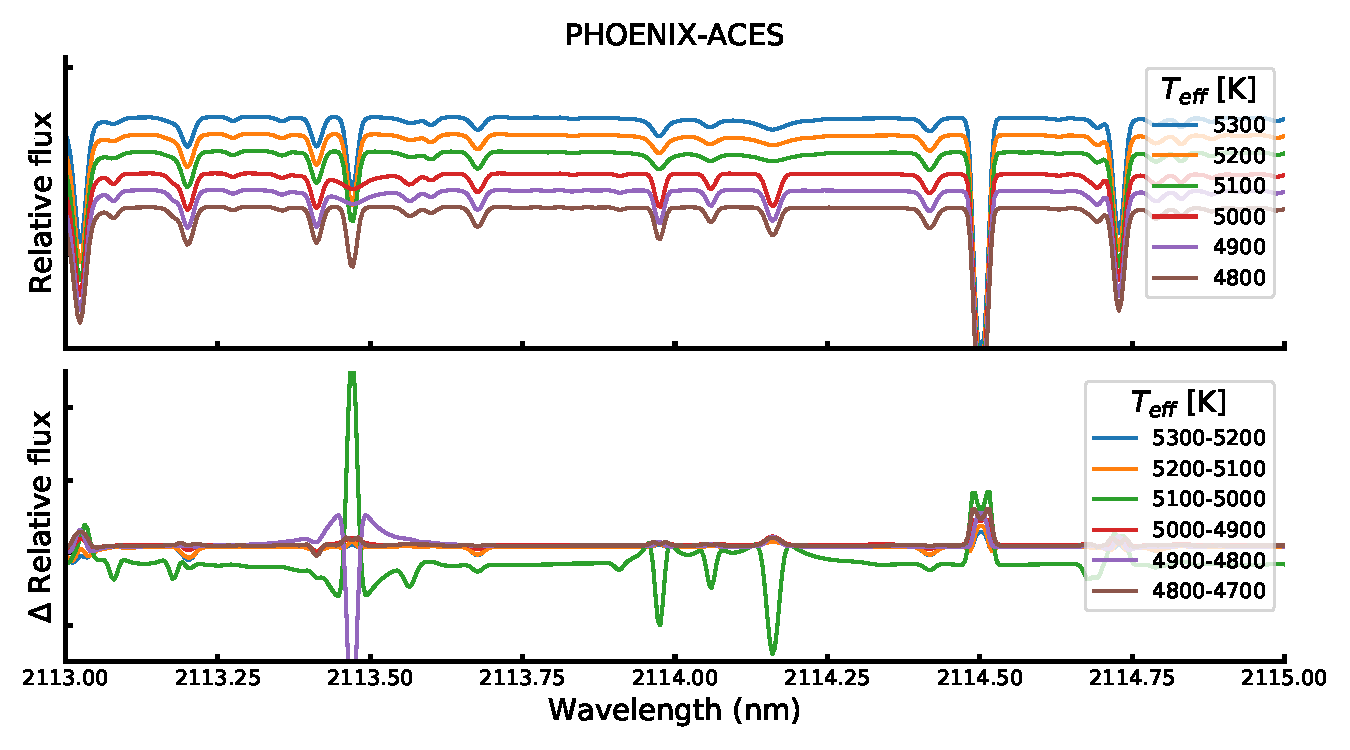
\includegraphics[width=0.8\linewidth]{figures/atmos_and_models/phoenix_differece_at_5000K}
    \caption[Difference in successive {PHOENIX-ACES} spectra around 5000\K.]{Top: Incremental {PHOENIX-ACES} model spectra between 4800--5300\K{} with \Logg{}=4.5 and \feh{}=0.0 fixed.
    Bottom: Difference in flux between successive models separated by 100\K{}.
    Apart from near absorption lines there is a discontinuity in the flux of the {PHOENIX-ACES} models between 5000 and 5100\K{}.}
    \label{fig:phoenixdiffereceat5000k}
\end{figure}


\subsection{BT-Settl}
\label{subsec:btsettl}
The {BT-Settl} models~\citep{allard_models_2012,allard_atmospheres_2012,rajpurohit_effective_2013,baraffe_new_2015}, are an evolution of both the \emph{DUSTY} and \emph{COND} models.
They are better suited for the entire range of {BD} temperatures down to 400\K{}, through hydrodynamical modelling of the mixing and settling of dust/clouds in the atmosphere of cool dwarfs~\citep{freytag_role_2010}.
The {BT-Settl} models now also include 3-D radiation transfer~\citep{seelmann_3d_2010}.

The {BT-Settl} are generally more difficult to work with due to their file format (in comparison to {PHOENIX-ACES}).
The most recent {BT-Settl} spectral library, using version 15.5 of the {PHOENIX} code, is designated {CIFIST2011\_2015}\footnote{\url{https://phoenix.ens-lyon.fr/Grids/{BT-Settl}/CIFIST2011_2015/}}~\citep{baraffe_new_2015} and includes newer~\citet{caffau_solar_2011} solar abundances and is combined with evolutionary modelling.
It is available in a fits format which is easier to use.
The parameter range available from the pre-computed library is given in \cref{tab:btsettl_params}.

%!TEX root = ../../thesis.tex

\begin{table}
    \centering
    \caption[{BT-Settl} parameter space.]{Full parameter space of the {BT-Settl} ({CIFIST2011\_2015}) spectral grid~\citet{baraffe_new_2015}.}
    \begin{tabular}{cr@{ -- }lc}    % Seperate columns with --
        \toprule
         & \multicolumn{2}{c}{Range}       & Step size\\
        \midrule
        \txteff{} [K]  &  1\,200 & 7\,000    & 100 \\
        \logg{}          &  2.5      & 5.5         & 0.5 \\
        \feh{}            & 0          & 0            & - \\    % Strange spacing of [ ] in table so added \ to all rows
        \(\alpha\)/Fe   &  0         & 0            & - \\
        \bottomrule
    \end{tabular}
    \label{tab:btsettl_params}
\end{table}


In this work the {BT-Settl} models used did not go below the {PHOENIX-ACES} limit of 2300\K{}, used as a comparisons.
Above this temperature there are some difference observed in the line strengths between the two models but their spectra are similar in the \nir{} (see \cref{subsec:phoenix_comparision}).


\subsection{Model access}
\label{subsec:model_access}
The pre-computed synthetic spectral libraries for the {PHOENIX-ACES} models (\cref{tab:phoenix}) are easily obtainable from \href{http://phoenix.astro.physik.uni-goettingen.de/}{http://phoenix.astro.physik.uni-goettingen.de/} while pre-computed models for the {BT-Settl} (\cref{tab:btsettl_params}) and other {PHOENIX} spectra can be found at \href{https://phoenix.ens-lyon.fr/Grids/}{https://phoenix.ens-lyon.fr/Grids/}.
A simulator is also available to generate {BT-Settl} spectra or other {PHOENIX} spectra from {Allard France} at \href{phoenix.ens-lyon.fr}{phoenix.ens-lyon.fr}, for specific parameters or abundances.

The spectral model libraries were downloaded using the above links and accessed using the ``grid tools'' interface provided in the \emph{Starfish}\footnote{\url{https://github.com/iancze/Starfish}} Python package~\citep{czekala_constructing_2015}.
The ``grid tools'' enables the fast, efficient, and simple loading of stellar spectra for use in the simulation performed in this work.
For instance a spectra from a given model can be loaded simply using the four values of identifying parameter values [\Teff{}, \Logg{}, \feh{}, \alphafe{}]\footnote{\feh{} and \alphafe{} are abundances of \ce{Fe} and \(\alpha\) elements relative to those in the Sun.
    The definition of the scale is \([X/H] = \log_{10}{\left(\frac{n_{\ce{X}}}{n_{\ce{H}}}\right)}_{\star} - \log_{10}{\left(\frac{n_{\ce{X}}}{n_{\ce{H}}}\right)}_{\odot}\), where $n_{\ce{X}}$ is the number of atoms of element \ce{X} and $n_{\ce{H}}$ is the number of atoms of Hydrogen.}.


\subsection{Comparing models}
\label{subsec:phoenix_comparision}
 \begin{figure}
    \centering
    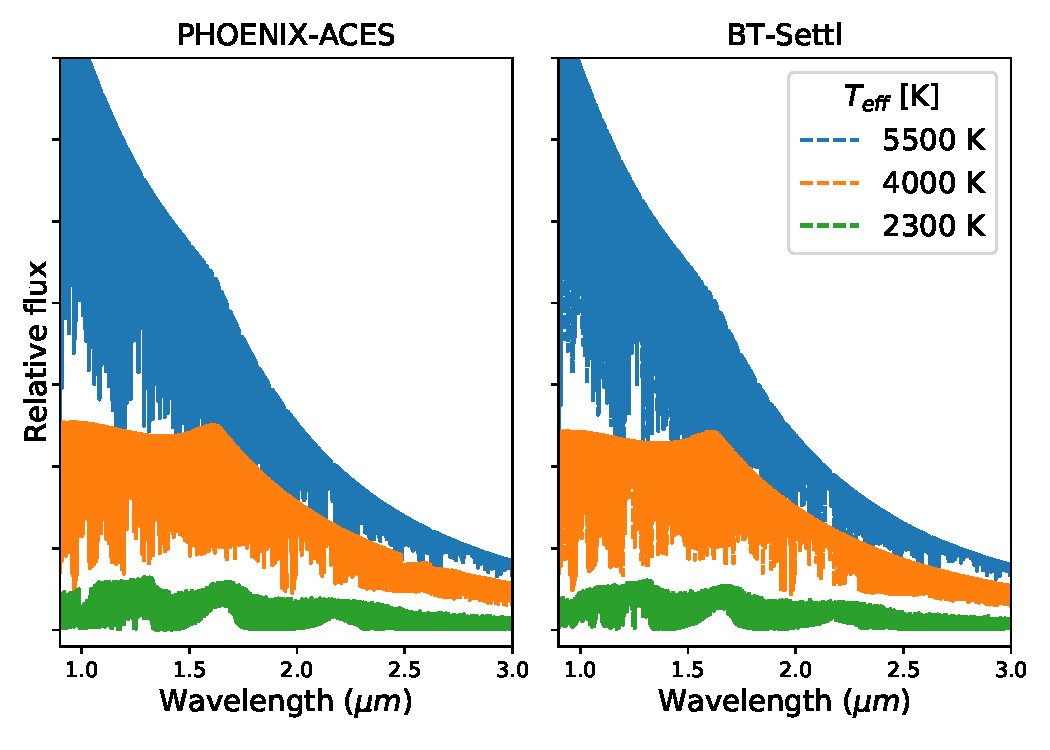
\includegraphics[width=0.6\linewidth]{figures/atmos_and_models/phoenix_large_scale_comparision}
    \caption[Large scale comparison between the {PHEONIX-ACES} and {BT-Settl} spectra.]{{PHOENIX-ACES} (left) and {BT-Settl} (right) spectra in the \nir{} wavelength region for three different temperature stars, \Logg{}=4.5, \feh{}=0.}
    \label{fig:phoenixlargescalecomparision}
\end{figure}

\begin{figure}
    \centering
    \begin{tabular}{cc}
        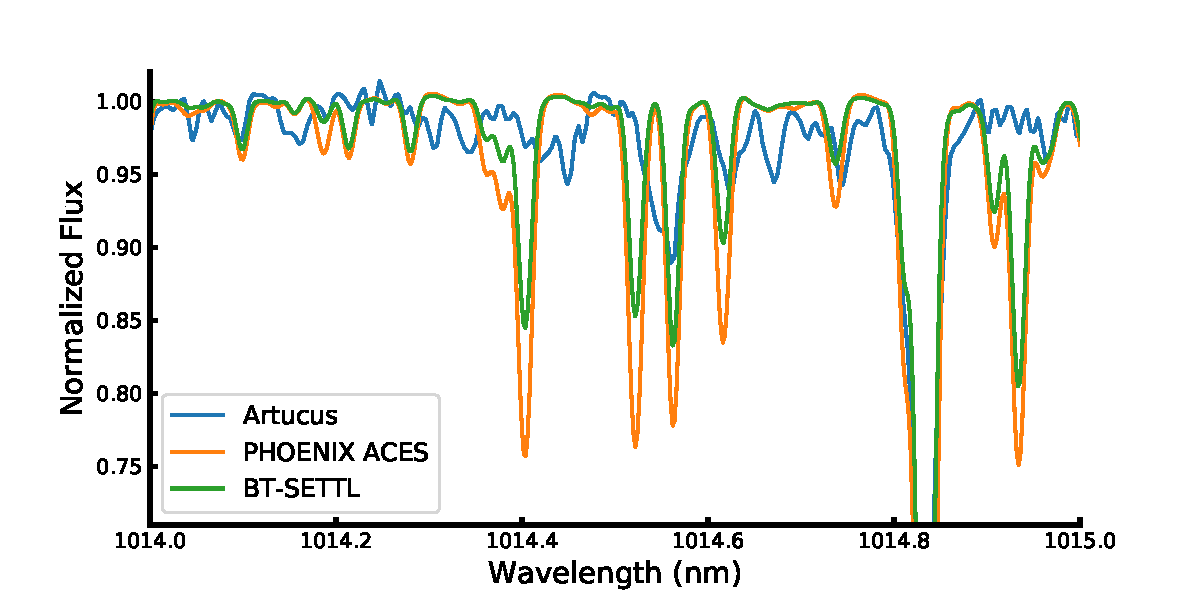
\includegraphics[width=0.48\linewidth]{figures/atmos_and_models/artucus_1micron} & 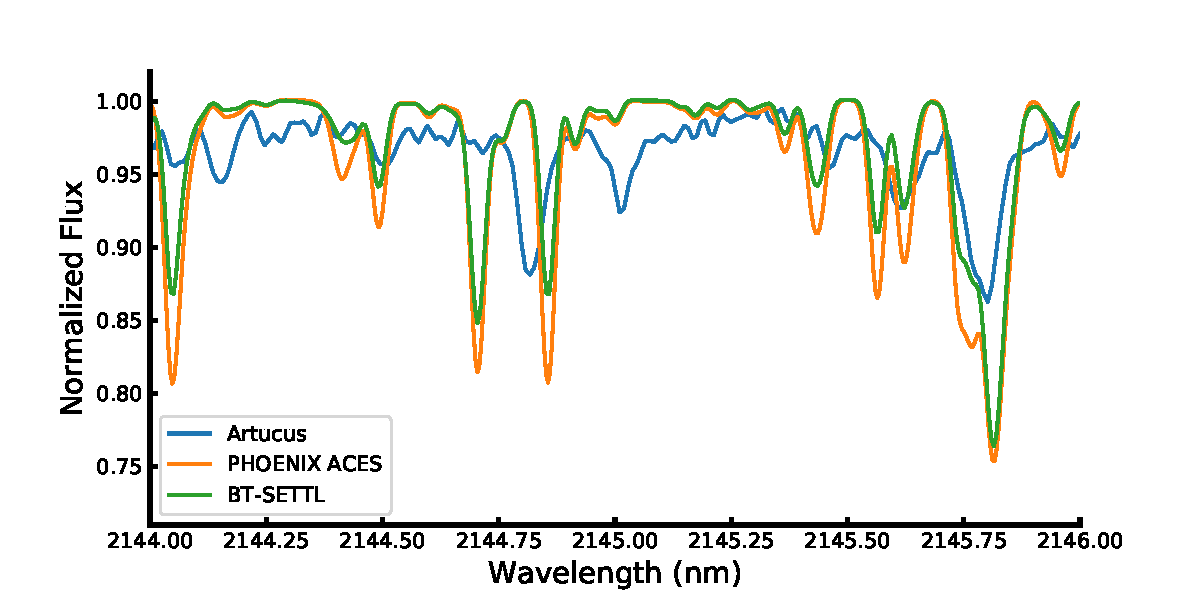
\includegraphics[width=0.48\linewidth]{figures/atmos_and_models/artucus_2micron}\\
    \end{tabular}
    \caption[Comparision of the spectrum of Arcturus to synthetic specta.]{Spectrum of Arcturus compared to synthetic spectra with the closest spectral parameters at wavelengths around 1014\nm{} (left) and 2145\nm{} (right).}
    \label{fig:artucus1-2micron}
\end{figure}

Here a comparison between the {PHOENIX-ACES} and {BT-Settl} spectra is briefly given.
\Cref{fig:phoenixlargescalecomparision} shows the model spectral flux in the \nir{} range of 0.9--3\um{} for three different stellar temperatures: 5500, 4000, and 2300\K{}.
At this large scale the spectra look fairly similar.

On closer inspection though, the spectra are slightly different with the {PHOENIX-ACES} spectra having deeper absorption lines compared to the {BT-Settl} models; however they do appear to have most of the same absorption lines.
This can be seen in \cref{fig:artucus1-2micron} which contains the {PHOENIX-ACES} and {BT-Settl} at two different regions in the \nir, 1013\nm{} and 2110\nm{}.
Temperature of both models is 4300\K{} while the \Logg{} is 1.5 for {PHOENIX-ACES} and 2.5 for {BT-Settl} (closest available) and the models are convolved to R=100,000.
This is in an attempt to match the parameters to the observations of {Arcturus} at R=100\,000 shown blue.
Cross-correlation and a Doppler shift has been used to align the model spectra to the observations.
There is a striking difference between the models and observations with several lines present in the models that are not seen in the real observation, while a few lines observed that are not seen in the models.
When the observed absorption lines do align with the models there is a difference in the depth of the lines.
These differences are primarily not from the differences between the model parameters actual stellar parameters which are small.
These differences are shown at two different wavelengths and reveal that there is still room for improvement in the synthetic models to match observed spectra in the \nir{} and at high resolution.
Spectral discrepancies in the {BT-Settl} models are noted by~\citet{rajpurohit_effective_2013}.

A further example of this is shown in \cref{fig:visualinspection-hd2118471} in which an observed {CRIRES} spectra is fitted with a binary model.
The flux ratio \FtwoFone{}=0.066 so the model is dominated by a single {PHOENIX-ACES} model, and shows several line discrepancies.
This caused issues with the fitting procedure in \cref{cha:model_comparison}.
\Cref{fig:crires-pop-mismatch} is a further example of the spectral differences at the \nir{} wavelengths specifically used in this work, in a spectra from (in reduced form) the CRIRES-POP library~\citep{lebzelter_crirespop_2012,nicholls_crirespop_2017}.
It shows differences between the CRIRES-POP \emph{K}-band spectra of {10\,Leo} and the {PHOENIX-ACES} spectrum with corresponding parameters (\txteff=4800, \Logg{}=3.00, \feh{}=0.0).


\begin{figure}
    \centering
    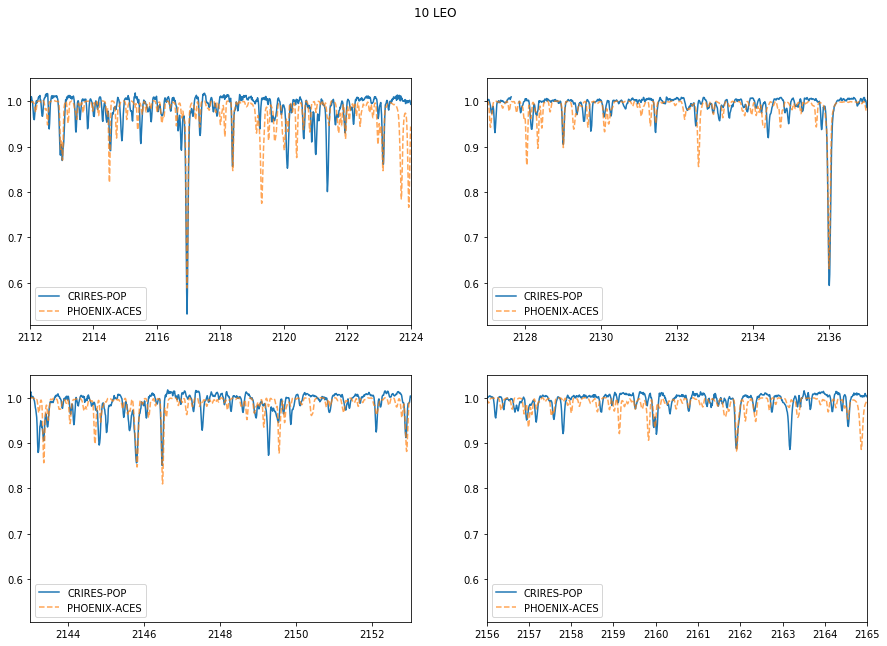
\includegraphics[width=0.8\linewidth]{figures/atmos_and_models/CRIRES-POP-mismatch}
    \caption[Comparision of the spectrum of {10\,Leo} to synthetic {PHOENIX-ACES} spectum.]{CRIRES-POP spectra of {10\,Leo} compared with a {PHOENIX-ACES} model for a CRIRES observation between 2112-2165\nm{}.}
    \label{fig:crires-pop-mismatch}
\end{figure}
% \todo{\cref{fig:crires-pop-mismatch} needs improved style}
